\documentclass[12pt]{article}
\usepackage{setspace,graphicx,amsmath,geometry,fontspec,titlesec,soul,bm,subfigure}
\titleformat{\section}[block]{\LARGE\bfseries}{\arabic{section}}{1em}{}[]
\titleformat{\subsection}[block]{\Large\bfseries\mdseries}{\arabic{section}.\arabic{subsection}}{1em}{}[]
\titleformat{\subsubsection}[block]{\normalsize\bfseries}{\arabic{subsection}-\alph{subsubsection}}{1em}{}[]
\titleformat{\paragraph}[block]{\small\bfseries}{[\arabic{paragraph}]}{1em}{}[]
\setmainfont{Times New Roman}
\renewcommand{\baselinestretch}{1.15}
\renewcommand\contentsname{Inhaltverzeichnis}
\geometry{a4paper,left=2.5cm,right=2.5cm,top=2.5cm,bottom=2.5cm}
\begin{document}
	\newpagestyle{main}{            
		\sethead{}{Kapitel 5}{} 
		\setfoot{}{\thepage}{}
		\headrule
		\footrule
			}
	\pagestyle{main}
\tableofcontents
\newpage
\section{Trasseneinrechnung und Absteckung im Straßen- und Gleisbau}	
\subsection{Straßenentwurf}
Trasse: Achse eines linienförmigen Objekts, horizontal festgelegt im Lageplan und vertikal festgelegt im Höhenplan. Beide Pläne sind miteinander abgestimmt.
\subsection{Entwurfselemente im Lage und Höhenplan}
\subsubsection{Krümmungsbild}
bei direktem Übergang, Gerade - Kreisbogen $\frac{dR}{dL} \sim \infty \longrightarrow$ Klothoid = Lineare Änderung der Krümmung $k = \frac{L}{A^2}$, $A:$ Klothoid Parameter.
\subsubsection{Gerade}
\subsubsection{Kreisbogen}
Radius $R \longrightarrow$ durch Fahrdynamik begrenzt. \newline
Länge $b \longrightarrow$ mindesten 2s zu durchfahren. \newline
\newline
Hauptpunkt: Bogenanfang(A), Bogenendpunkt(E), Kreismittelpunkt(M) \newline
\begin{itemize}
\item Zentriwinnkel des Bogens $r$
\item $\b = R \cdot r$
\item $r = \frac{b}{R}$
\item Tangentenlänge: $t = R \tan \frac{r}{2}$
\end{itemize}
Bestimmung von Zwischenpunkten:
\begin{equation*}
r' = \frac{b'}{R}
\end{equation*}
$b'$ wird vorgegeben, z.B. alle 10m
\begin{gather*}
x_P = R \cdot \sin(r') \\
y_P = R \cdot \cos(r')
\end{gather*}
\begin{figure*}[ht]\centering
	\subfigure[]{
		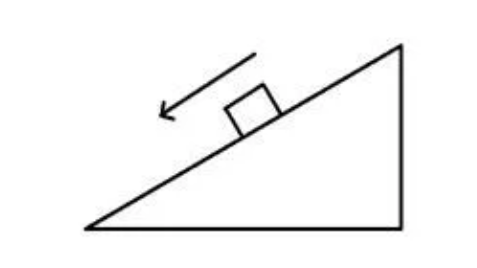
\includegraphics[width=0.65\textwidth]{phisik.png}}
\end{figure*}
\begin{gather*}
G = m \cdot g \\
F = \frac{mv^2}{R} \\
G_N = G\cos \alpha = mg \cos \alpha \\
G_R = G \sin \alpha \\
F_R = F \cos \alpha = m \frac{v^2}{R} \cos \alpha \\
\end{gather*}
Forderung(damit das auf der Straße bleiben)
\begin{gather*}
G_R + f_R(G_N + F_N) \geq F_R \\
mg \sin \alpha + f_R mg \cos \alpha + f_R m \frac{v^2}{R} \sin \alpha \geq m\frac{v^2}{R} \cdot \cos \alpha \\
\alpha\; klein \longrightarrow \sin \alpha \approx \tan \alpha \approx q \\
\cos \alpha \approx 1 \\
\cdots \\
R \geq \frac{(1-f_R \cdot q)}{q + f_R} \cdot \frac{v^2}{g}
\end{gather*}
Beispiel: $v = 100km/h$, $q=6\%$, $f_R = 0,4 \longrightarrow R > 167m$ als minimalradius.\newline
Seitenbeschleunigung bei der Kreisfahrt: \newline
Kriterium des Fahrkomfortarts: \newline
$p$: Seitenbeschleunigung.
\begin{gather*}
p = \frac{F_R - G_R}{m} = \frac{v^2}{R} (\cos \alpha - g \sin \alpha) \\
p = \frac{v^2}{R} - q \cdot g \\
empirische\; Grenzwert: p = 0,85m/s^2
\end{gather*}
Forderung:
\begin{gather*}
\frac{v^2}{R} - g \cdot q \leq 0,85 \\
\frac{v^2}{R} \leq 0,85 + g \cdot q \\
R \geq \frac{v^2}{0,85 + g \cdot q} \\
v = 100km/h \quad q=6\% \longrightarrow R>543m
\end{gather*}
Kriterium Fahrkomfort ist entscheidend \newline
\newline
Pfeilhöhenverfahren: \newline
Ermittelung der Krümmung aus drei Punkten bei vorausgesetzten Kreisbogen (bzw. des Radius)
\begin{figure*}[ht]\centering
	\subfigure[h:Pfeilhöhe, s:Sehnenlänge]{
		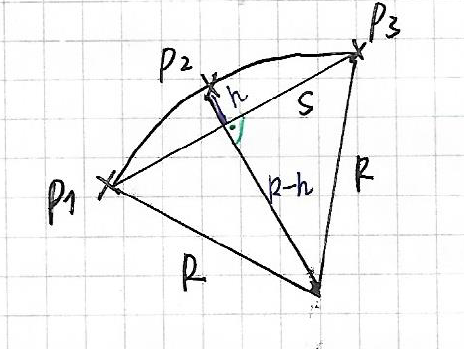
\includegraphics[width=0.65\textwidth]{Kreis.png}}
\end{figure*}
\begin{gather*}
R^2 = (R-h)^2 + (\frac{S}{2})^2 \\
R^2 = R^2 - 2Rh + h^2 + (\frac{S}{2})^2 \\
\cdots \\
k = \frac{1}{R} = \frac{8h}{s^2}
\end{gather*}
Radius somit graphisch bestimmbar. 
\subsubsection{Klothoide}
Hauptpunkte:
\begin{itemize}
\item ÜA: Klothoideanfang
\item ÜE: Klothoideende
\end{itemize}
gegeben: $R$, $A$, $x_A$, $y_A$ \newline
gesucht:
\begin{itemize}
\item $L$: Bogenlänge
\item $\tau$: Tangentenwinkel
\item $t_A$, $t_E$: Tantentenlänge
\item $x_E$, $y_E$: Koordinaten des Klothoidenpunktes
\item $\Delta R$: Tangentenabrückung
\end{itemize}
Bogenlänge $L = \frac{A^2}{R}$ \newline
\newline
für einen laufenden Punkt $P'$: 
\begin{gather*}
k' = \frac{1}{R'} = \frac{L'}{A^2}\\
dL = R \cdot d \tau \\
\longleftrightarrow d \tau = \frac{L'}{A^2} dl \\
\tau = \int_{ÜA}^{ÜE} d \tau = \int_{ÜA}^{ÜE} \frac{L'}{A^2} dL \\
\tau = \frac{L}{2R} \\
L = \frac{A^2}{R} \longleftrightarrow \tau = \frac{L^2}{2A^2}
\end{gather*}
Koordinaten $x_E$, $y_E$, wieder kleine Änderung für laufende Punkt.
\begin{gather*}
dy = dL \sin \tau \\
dx = dL \cos \tau \\
y_E = \int_{ÜA}^{ÜE} dy = \int_{ÜA}^{ÜE} dL \sin \tau \\
x_E = \int_{ÜA}^{ÜE} dx = \int_{ÜA}^{ÜE} dL \cos \tau \\
y_E = \int_{ÜA}^{ÜE} \sin (\frac{L^2}{2A^2}) dL \\
x_E = \int_{ÜA}^{ÜE} \cos (\frac{L^2}{2A^2}) dL \\
\end{gather*}
Fresnel'sche Integral:
\begin{itemize}
\item nicht geschlossen lösbar
\item Reihenentwicklung 
\end{itemize}
für Einheitsklothoide 
\begin{gather*}
l=\frac{L}{A}, \quad r=\frac{R}{A} \\
\longleftrightarrow L = A \cdot l,\quad R = A \cdot r \\
Y_E = \int_{ÜA}^{ÜE} \sin(\frac{l^2}{2}) A dl = A y_E \\
X_E = \int_{ÜA}^{ÜE} \sin(\frac{l^2}{2}) A dl = A x_E 
\end{gather*}
Reihenentwicklung 
\begin{gather*}
x_E = l - \frac{l^5}{40} + \frac{l^9}{3456} \\
y_E = \frac{l^3}{6} - \frac{l^7}{336} + \frac{l^{11}}{42240}
\end{gather*}
Dann:
\begin{gather*}
X_E = A \cdot x_E \\
Y_E = A \cdot y_E \\
\end{gather*}
Tangente Länge $t_A$, $t_E$:
\begin{gather*}
t_A = X_E - Y_E \cot (\tau) \\
t_E = \sqrt{(X_E - t_A)^2 + Y_E^2}
\end{gather*}
Tangentabrücklung
\begin{gather*}
R + \Delta R = R \cos \tau + Y_E \\
\Delta R = Y_E - R (1 - \cos \tau)
\end{gather*}
Zusätzliche Elemente 
\begin{gather*}
s = \sqrt{X_E^2 + Y_E^2} \\
bei\; X_A = 0, \; Y_A = 0
\end{gather*}
\begin{equation*}
\sigma = \arctan(\frac{Y_E}{X_E})
\end{equation*}
Mittelpunkt des Folgekreises
\begin{gather*}
X_M = X_E - R \sin \tau \\
Y_M = Y_E + R \cos \tau
\end{gather*}
Berechnung von Zwischenpunkten $\longrightarrow$ Übergang auf Einheitsklothoide,
\begin{gather*}
l' = \frac{L'}{R} \\
x_P = l' - \frac{l'^5}{40} + \frac{l'^9}{3456} \\
y_P = \frac{l'^3}{6} - \frac{l'^7}{336} + \frac{l'^{11}}{42240} \\
X_P = R x_P \\
Y_P =R y_P
\end{gather*}
Seitenrück bei der Klothoidenfahrt \newline
Änderung der Seitenbeschleunigung über die Zeit: $r = \frac{dp}{dt}$, mit $p=$ Seitenbeschleunigung. $r \leq 0,5$ bis $0,7m/s^2$ (empirische Grenzwert) 
\begin{equation*}
r = \frac{dp}{dt} = \frac{dp}{dR} \cdot \frac{dR}{dL} \cdot \frac{dL}{dt}
\end{equation*}
(a). $\frac{V^2}{R} - g \cdot q$, bei Plannung $q$ kompensiert $\frac{1}{3}$ der Fliehkraft.
\begin{equation*}
p = \frac{2}{3} \frac{v^2}{R} \longrightarrow \frac{dp}{dr} = - \frac{2}{3} \frac{v^2}{R^2}
\end{equation*}
(b). 
\begin{gather*}
k = \frac{1}{R} = \frac{L}{A^2} \longleftrightarrow R = \frac{A^2}{L} \\
\frac{dR}{dL} = - \frac{A^2}{L^2} = - \frac{R^2}{A^2} \\
da \; L^2 = \frac{A^4}{R^4}
\end{gather*}
(c). 
\begin{gather*}
\frac{dL}{dt} = v
\end{gather*}
$(a) + (b) + (c) \longrightarrow r = - \frac{2}{3} \frac{V^2}{R^2}(-(\frac{R^2}{A^2}) v) = \frac{2}{3} \frac{V^3}{A^2} \leq 0,5 m/s^3 \longrightarrow A \geq \sqrt{\frac{2}{3 \cdot 0,5} v^3} = \sqrt{\frac{4}{3} v^3}$ \newline
Numerische Beispiel: $v = 100km/h \longrightarrow A > 170m$
\subsubsection{Weitere Übergangsbogen}
Nutzung nur bei der Gleislaussierung, da beide Klothode an den Punkten ÜA und ÜE ein Sprung im Rückauftritt. \newline
1) Parabel 5. Grades / Bloss - Kurve
\begin{gather*}
y = \frac{x^4}{4 \cdot r \cdot l} - \frac{x^5}{10 \cdot r \cdot l^3} \\
k = \frac{3 \cdot x^2}{r \cdot l} - \frac{2 \cdot x^3}{r \cdot l^4}
\end{gather*}
2) Sinusoide \newline
Steige Verlauf des Seitenrucks, fahrdynamisch das Beste, Einsatz bei Magnetischwebebahn
\begin{gather*}
k = \frac{1}{R} (\frac{l}{L} - \frac{1}{2\pi} \sin (\frac{l'}{L} 2\pi))
\end{gather*}
\subsubsection{Überhöhung, Quer und Längsneigung}
Überhöhung: Höhendifferenz zwischen Innere und äußere Schiene; Angabe in mm(zwischen 20 und 180 mm) nur im Gleisbau. \newline
Neigungsmaße: \newline
\begin{itemize}
\item Neigungswinkel: $\alpha =  \arctan (\frac{\Delta H}{s})$
\item Prozent: p = $\frac{\Delta H}{s} \cdot 100\%$
\item Böschungsverhältnis: $\tan \alpha = \frac{1}{x} = \frac{\Delta H}{s}$ 
\end{itemize}
Steigung des Gelände von 1m der Entfernung von x. \newline
\newline
Querneigung: Überhöhung im Straßenbaus, Angabe in $\%$
\begin{itemize}
\item Mindestwerte zur Abführug des Oberflächenwassers (wenn kein Längsneigung): $2,5 \%$
\item Maximalwerte bei Kreisbögen: $5$ bis $8\%$
\item bei vier spruigen Straßen: Dachprofil
\item Verwindung: Drehen der Querschnitt von der Achse; meist in Übergangsbögen.
\end{itemize}
Längsneigung: \newline
Straßenbau:
\begin{itemize}
\item Maximalwerte Straßenbau: $4,5 - 8\%$
\item Mindestwerte Straßenbau:(zum Abfluss der Oberflächenwassers) $0,7 - 1\%$
\end{itemize}
Gleisbau: 
\begin{itemize}
\item Maximalwerte beim Gleisbau: $1,25\%$ bei Hauptbahnen, $4\%$ bei S-Bahnen und Nebenbahnen, $0,25\%$ in Bahnhöfen.
\end{itemize}
\subsubsection{Kippen und Wannenausführung}
Steigung: positiv: \textcircled{+} S \newline
Gefälle: negativ: \textcircled{-} S \newline
Wannenhalbmesse: \textcircled{+} H \newline
Kuppenhalbmesse: \textcircled{-} H \newline
\begin{gather*}
\tan \alpha = \frac{s_1}{100} \approx \alpha \qquad(positiv) \\
\tan \beta = \frac{s_2}{100} \approx \beta \qquad (negativ) \\
T_{\alpha} = -H \cdot \frac{S_1}{100} \\
T_{\beta} = -H \cdot \frac{-S_2}{100} \\
2T = T_{\alpha} + T_{\beta} = H(\frac{S_2 - S_1}{100}) \\
T = T_{\alpha} + T_{\beta} = \frac{H}{2}(\frac{S_2 - S_1}{100}) \\
S(x) = S_1 + \frac{x}{H} \cdot 100 \\
y(x) = \frac{s_1}{100}x + \frac{x^2}{2H} \\
f = \frac{x_M^2}{2H} = \frac{T^2}{2H} \\
f = \frac{H}{8} \frac{(s_2 - s_1)^2}{100^2} \\
h_a = \frac{(S_H^a)^2}{2H} \\
h_z = \frac{(S_H^z)^2}{2H} \\
\longrightarrow S_H^{a} = \sqrt{h_a \cdot 2H} \\
S_H^z = \sqrt{h_z \cdot 2H} \\
S_H = \sqrt{h_a \cdot 2H} + \sqrt{h_z \cdot 2H} \\
S_H^2 = 2H (\sqrt{h_a} + \sqrt{h_z})^2 \\
H = \frac{S_H^2}{2 (\sqrt{h_a} + \sqrt{h_z})^2} \\
h_a = 1m \\
h_z = f(v)\; mit \; 0m\; bei\; v=60km/h \\
0,45m\; bei\; v=130km/h
\end{gather*}
numerische Beispiel
\begin{gather*}
V = 100km/h \longrightarrow S_H = 170m \longrightarrow V_{Kuppe} \geq 8300m \\
H_{Wanne} = \frac{H_{Kuppe}}{2}\quad (nur\; aus\; optische\; Gründen)
\end{gather*}
\subsection{}
\subsubsection{Eilinie}
Folge: Kreisbogen - Klothoide - Kreisbogen \newline
$\longrightarrow$ Klothoide zwischen 2 gleichsinnig gekrümmten Kreisbögen. (mit unterschiedlichen Radien) \newline
$k_1 = \frac{1}{R_1}$, (ÜA) \newline 
$k_2 = \frac{1}{R_2}$, (ÜE) \newline
gegeben: $R_1$, $R_2$, $x_{m_1}$, $y_{m_1}$, $x_{m_2}$, $y_{m_2}$ \newline
Vorbedingungen:
\begin{itemize}
\item $R_1 > R_2$ 
\item $R_2$ innerhalb von $R_1$
\item $M_1$ und $M_2$ nicht identisch.
\end{itemize}
a: kürzester Abstand der verlängerten Kreisbögen / Kreisbogenabrückung. \newline
$a = R_1 - R_2 - \sqrt{(x_{m_1} - x_{m_2})^2 - (y_{m_1} - y_{m_2})^2}$ \newline
Klothoide Parameter $A_{E_i}$ \newline
\begin{gather*}
A_{E_i} = \sqrt[4]{24aR^3} \\
R = \frac{R_1 R_2}{R_1 - R_2} \\
L_{E_i} = \frac{A_E^2}{R}
\end{gather*}
$A_{E_i}$ stellt Näherungslösung, daher benötigt man eine iteration Vorgehesweise \newline
Iteration
\begin{itemize}
\item mit $A_{E_i}$ (als Nahrung) Koordinaten der Mittelpunkt berechnen. 
\item dann $a$ neu berechnen, und $A_{E_i}$
\item Korrektur von $a$ bzw. $A_{E_i}$ bis keine Wiedersprüche in dem Koordinaten auftreten.
\end{itemize}
\subsubsection{Wendelinie}
Kreis - Wendeklothoide - Kreis 
\begin{itemize}
\item Klothoide verbindert 2 Kreisbögen entgegengesetzte Krümmung 
\item kann auch als 2 Entgegengesetzte gekrümmte Klothoide aufgefasst werden
\item am Wendepunkte gleiche Tangente
\item Klothoidenparameter sollten bei beide Ästen gleich sein oder maximal $0,07 \leq A_1/A_2 \leq 1,5$ sein. 
\end{itemize}
gegeben: $R_1$, $R_2$, $x_{m_1}$, $y_{m_1}$, $x_{m_2}$, $y_{m_2}$
\begin{gather*}
a = \overline{M_1 M2} - R_1 - R_2 \\
A_w = \sqrt[4]{24aR^3} \qquad (ohne\; Beweis)\\
R = \frac{R_1 R_2}{R_1 + R_2} \\
L_w = \frac{A_w^2}{R} \\
\Longrightarrow L_{w_1} = \frac{A_w^2}{R_1} \qquad L_{w_2} = \frac{A_w^2}{R_2} \\
y_{m_1} = R_1 + \Delta R_1 \quad mit\; \Delta R_1 = \frac{L^2 w_1}{24 R_1} \\
y_{m_2} = R_2 + \Delta R_2 \quad mit\; \Delta R_2 = \frac{L^2 w_2}{24 R_2} \\
x_{m_1} = x_{E_1} - R_1 \sin \tau_1 \quad mit \; \tau_1 = \frac{L_{w_1}}{2R_1}\\
x_[m_2] = x_{E_2} - R_2 \sin \tau_2 \quad mit \; \tau_2 = \frac{L_{w_2}}{2R_2}\\
\varepsilon = \arctan (\frac{x_{m_1} + x_{m_2}}{y_{m_1} + y_{m_2}})
\end{gather*}
$\Longrightarrow$ Bestimmung von $\overline{M_1 M_2}$ möglich \newline
Iteration (Da $A_w$, $\Delta R_1$, $\Delta R_2$ sind Nährungswerte)
\begin{itemize}
\item Berechnung von Kreismittelpunkten, die nicht mit Vorgabe übereinstimmen. 
\item $a$ / $A_w$ konvergieren
\item Berechnung von Kreismittelpunkten bis keine Wiedersrüche auftreten.
\end{itemize}
\subsubsection{Scheitelklothoide}
2 Klothoiden mit unterschiedlichen Vorzeichen der Krümmungsänderung grenzen ohne Kreisbogen aneinander. (Schlechte Fahrdynamik, da "Kreisbogendurchfahrt" in jedem Fall < 2,5), möglichst nicht verwenden! 
\subsection{Relation zwischen Höhen und Lageplan}
\subsection{Trasseneinrechnung nach graphischen Entwurf}
\subsection{Trassenlage und Höhenabsteckung}
\subsubsection{Lageabsteckung}
Tangentenpolygon berechnen. \newline
Beispie: Gerade - Klothoide - Kreisbogen 
\begin{itemize}
\item Vorgabe $x_A$, $y_A$, $t_{AE}$
\item $L$ bekannt
\item polares Anhängen für $x_E = (x_{Uea})$, $y_E = {y_{Uea}}$
\item $t_A$, $t_E$ $\tau$ aus Formel
\item Polares Anhängen von $x_{k_1}$, $y_{k_1}$ unter Nutzung von $t_A$
\item $t_{k_1, k_2} = t_{AE} - \tau$
\item Polares Anhängen von $x_{Uee} = (x_{k_A})$, $y_{Uee} = (y_{k_A})$ unter Nutzung von $t_E$ 
\item $t$, $j$ aus Formeln zum Kreisbogen.
\item Polares Anhängen von $x_{k_2}$, $y_{k_2}$ unter Nutzung von $t$
\item $t_{k_2 k_E} = t_{k_1 k_2} - \tau$
\item Polares Anhängen von $x_{k_E}$, $y_{k_E}$ unter Nutzung von $t$
\end{itemize}
\subsection{Trassenlage und Höhenabsteckung}
\subsubsection{Polare Absteckung}
\begin{itemize}
\item Tangenten Polygon in Landeskoordinaten berechnen
\item Berechnung der Bogenkleinpunkt (zwischenpunkte) bezogen auf Tangenten
\item Transformation der Zwischenpunkte in das Landessystem (3 Parameter (kein Maßstab))
\item Anlage aus trassennahem Polygons/Festpunkt
\item Polare Absteckung der Haupt- und Zwischenpunkt
\end{itemize}
\subsubsection{Orthogonale Absteckung}
\begin{itemize}
\item Tangenten Polygon in Landeskoordinaten berechnen (identisch)
\item Berechnung der Bogenkleinpunkt (zwischenpunkte) bezogen auf Tangenten (identisch)
\item Herstellung des Tangentpolygons in der Örtlichkeit
\item Orthogonale Absteckung der Zwischenpunkte
\end{itemize}
\subsubsection{Höhenabsteckung}
\begin{itemize}
\item alle Trassenpunkten werden zunächst ohne Höheninformation abgesteckt.
\item In Trassennähe wird dann an Absolutehöhe vermarkt
\item Von dort können die Höhen für übertragen und entsprechend Erdmassen entnommen oder aufgeschüttet werden
\end{itemize}
Höhenfeinabsteckung für Fahrbahnschnitt
\begin{itemize}
\item Nutzung des Leitdrahts (auch für die Lage)
\item Längsneigung wird gleichfalls durch Leitdrahts festgelegt
\item Querneigung wird angeschrieben
\item Heute werden Leitdraht oft durch komplett automatisiert Baumaschine und Soll-DGMs ersetzt. 
\end{itemize}
\end{document}
